\documentclass[11pt,a4paper]{article}
\usepackage[T1]{fontenc}
\usepackage[utf8]{inputenc}
\usepackage{lmodern,microtype}
\usepackage{amsmath,amssymb,amsthm,mathtools,bm}
\usepackage{booktabs,array,tabularx,longtable}
\usepackage{graphicx,float,caption}
\usepackage{xcolor}
\usepackage[margin=20mm]{geometry}
\usepackage{enumitem,fancyhdr}
\usepackage[hidelinks]{hyperref}
\hypersetup{
 unicode=true,
 pdftitle={FIN ST106--ST117: Projection Selection, Recovery, and Adversarial Lifts},
 pdfauthor={Krzysztof Żuchowski},
 pdfsubject={Analytical and computational execution of FIN programs ST106--ST117},
 pdfkeywords={FIN, observable algebra, lift spectrahedron, Krawczyk, Petz recovery, selector, Chernoff information, projection falsification}
}
\setlength{\parindent}{0pt}
\setlength{\parskip}{0.48em}
\setlength{\emergencystretch}{2em}
\setlength{\headheight}{14pt}
\setlist[itemize]{leftmargin=1.55em,itemsep=0.14em,topsep=0.2em}
\setlist[enumerate]{leftmargin=1.75em,itemsep=0.14em,topsep=0.2em}
\pagestyle{fancy}\fancyhf{}
\lhead{FIN ST106--ST117}\rhead{Release 10.63}\cfoot{\thepage}
\newtheorem{theorem}{Theorem}[section]
\newtheorem{proposition}[theorem]{Proposition}
\newtheorem{corollary}[theorem]{Corollary}
\newcommand{\proven}{\textcolor{green!40!black}{\textbf{[PROVEN]}}}
\newcommand{\strong}{\textcolor{blue!70!black}{\textbf{[STRONG EVIDENCE]}}}
\newcommand{\conditional}{\textcolor{violet!65!black}{\textbf{[CONDITIONAL]}}}
\newcommand{\openstatus}{\textcolor{red!72!black}{\textbf{[OPEN]}}}
\newcommand{\statusboundary}{\textcolor{orange!80!black}{\textbf{[BOUNDARY]}}}
\newcommand{\resultbox}[1]{\begin{center}\fcolorbox{blue!60!black}{blue!4}{\parbox{0.92\textwidth}{#1}}\end{center}}

\begin{document}
\pagenumbering{gobble}
\begin{titlepage}
\centering
\vspace*{1.0cm}
{\LARGE\bfseries FIN ST106--ST117\par}
\vspace{0.32cm}
{\Large Projection Selection, Recovery, and Adversarial Lifts\par}
\vspace{0.42cm}
{\large Observable-algebra no-go theorems, facial geometry of the 78-dimensional lift fiber, a transcendental-kernel fold certificate, maximal recoverable codes, equivariant nonselection, passive antisymmetric memory, robust Chernoff design, refinement twists, and adversarial projection alternatives\par}
\vspace{0.85cm}
{\Large Krzysztof \.{Z}uchowski\par}
\vspace{0.20cm}
{\large Independent Researcher --- Fractal Information Theory Project\par}
{\large ORCID: 0009-0002-0909-3613\par}
\vspace{0.65cm}
{\large FIN Release 10.63 --- Version 1.0.0\par}
{\large August 11, 2026\par}
\vfill
\begin{minipage}{0.91\textwidth}
\textbf{Question.} Can the projection interpretation be selected by symmetry or locality, can its lost information be recovered, and can its nonidentifiability be closed by proof-grade certificates rather than favorable examples?\par
\textbf{Methods.} Finite $C^*$-algebras, Schur commutants, convex spectrahedra, parametric interval Krawczyk operators, Knill--Laflamme error correction, equivariant probability, passive realization theory, Chernoff geometry, directed refinement categories, and adversarial lift construction.\par
\textbf{Epistemic rule.} ``Observable reality is a projection of FIN'' is retained only as a counterfactual hypothesis. Exact finite mathematics is not promoted to experimentally established physics.\par
\textbf{Repository snapshot.} Audited tracked base commit \texttt{8a4c9b0b29b4fed8f7dcdc86e79b98306818efea}; Release 10.63 artifacts are additional local files identified by the SHA-256 manifest.\par
\textbf{Repository.} \url{https://github.com/hyconiek/Fractal-Nadsoliton-Theory}\par
\textbf{License.} CC BY 4.0.
\end{minipage}
\end{titlepage}
\pagenumbering{arabic}

\begin{abstract}
ST106--ST117 close several questions left open by Release 10.62 and sharpen the boundary of the projected-universe interpretation. ST106 proves that layer-swap symmetry leaves the algebra $M_{12}\oplus M_{12}$, not the desired coarse-visible/fine-blind algebra $M_{12}\oplus\mathbb C$. The latter follows only after invariance under every fine-sector unitary is imposed; this is precisely an added fine-blindness premise. ST114 independently proves that ordinary vertex locality moves in the opposite direction: vertex projectors and a connected graph generator produce the full algebra $M_{24}$. Therefore neither symmetry nor locality selects the projection algebra.

ST107 identifies the recession cone of the complete lift spectrahedron as the nonnegative diagonal orthant. It has twelve rank-one extreme rays, and $B=A$ is an exact vertex. ST117 turns those rays into noncirculant adversarial lifts
\[
L_{i,t}=PAP^*+F(A+tE_{ii})F^*,\qquad t\ge0,
\]
which preserve every conditioned coarse functional-calculus record but are detected by one fine-site observable. The nonidentifiability is consequently structural, not an accident of the earlier one-parameter dyadic family.

ST108 strengthens the previous fold certificate. Direct interval evaluation of
\[
K(d)=\frac{\cos(0.18575d+0.16250)}{1+d^{9/5}}
\]
is propagated through the full 15-variable Krawczyk calculation. A radius-$10^{-8}$ box has strict inclusion margin $9.9999871\times10^{-9}$. Uniform parametric inclusion proves that every operator in the exact-decimal transcendental interval family has a unique fold root inside the common box. This is a source-code interval theorem, not a proof-assistant theorem or a physical bifurcation measurement.

ST109 proves that coarse/fine pinching has recoverable quantum codes of maximal dimension twelve. ST110 proves that the unique $C_{12}$-invariant branch probability is uniform and therefore nonselecting. ST111 proves that one antisymmetric memory block generates oscillatory phase but remains passive under collocated ports. ST112 gives a conditional numerical design for hidden-$q$ discrimination. ST113 classifies spin twists on the directed refinement category and shows that every nontrivial fine holonomy remains newly supplied data.

ST115 closes the full independent uniform-contamination rectangle left open in ST103. Joint concavity of the Chernoff coefficient, strict convexity in the Chernoff exponent, an interval-isolated stationary point, and strictly positive envelope derivatives prove that $(\epsilon_P,\epsilon_Q)=(0.12,0.12)$ is the global worst corner for the frozen synthetic probability tables. ST116 does not manufacture a thermal separation: it proves that ``outside thermal operations'' is under-typed until the admissible bath and dilation class is declared. The cumulative result is a more rigorous projection model and a stronger no-go boundary: the projection can be analyzed and falsified conditionally, but strict FIN still does not select its observable algebra, branch, apparatus, clock, or physical scale.
\end{abstract}

\textbf{Status vocabulary.} \proven{} is an exact analytic, finite, or source-code interval result in its stated scope. \strong{} is reproducible numerical evidence. \conditional{} requires displayed additional resources. \openstatus{} marks an attempted target not closed. \statusboundary{} states a non-implication.

\tableofcontents
\newpage

\section{Frozen mathematical core and scope}

The strict working operator is kept separate from the legacy intermediate bridge kernel. On $C_{12}$,
\begin{equation}
W_{xx}=0,\qquad
W_{xy}=\frac{\cos(0.18575d(x,y)+0.16250)}{1+d(x,y)^{9/5}}\quad(x\ne y),
\qquad A=sI-W,
\label{eq:strict}
\end{equation}
where $s=\sum_yW_{xy}$. Hence
\[
\langle f,Af\rangle=\frac12\sum_{x,y}W_{xy}|f_x-f_y|^2\ge0
\]
for the declared positive edge weights. The coarse/fine isometries are
\[
P=\frac1{\sqrt2}\binom{I}{I},\qquad F=\frac1{\sqrt2}\binom{I}{-I},
\qquad P^*P=F^*F=I,\quad P^*F=0.
\]
Every real symmetric lift satisfying $LP=PA$ has the block form
\begin{equation}
L=PAP^*+FBF^*.
\label{eq:lift}
\end{equation}
For graph-Laplacian sign and positivity constraints, ST95 obtained
\begin{equation}
B\succeq0,\qquad B_{ii}\ge A_{ii},\qquad A_{ij}\le B_{ij}\le-A_{ij}\quad(i\ne j).
\label{eq:fiber}
\end{equation}

\resultbox{\textbf{Main conclusion.} The proposed fine-blind algebra is not selected by layer symmetry and is contradicted by unrestricted vertex locality, which generates too many observables. The hidden lift set also contains twelve unbounded adversarial directions. Projection is therefore a precise conditional operational model, not a strict consequence of the current kernel.}

\subsection*{Kernel and physics discipline}

The legacy ontological kernel remains an intermediate bridge kernel. No legacy physical role is transferred to~\eqref{eq:strict}; no completion theorem is claimed. All calculations are finite and dimensionless. They provide no dimensional clock, SI scale, environment, apparatus, laboratory record, Standard Model, gravitation, $L_{\rm total}$, or ToE closure. The selector obstruction QW-2191 remains open.

\section{Outcome matrix}
\small
\begin{longtable}{@{}p{0.065\textwidth}p{0.27\textwidth}p{0.27\textwidth}p{0.31\textwidth}@{}}
\toprule ID & Target & Outcome & Boundary\\\midrule\endfirsthead
\toprule ID & Target & Outcome & Boundary\\\midrule\endhead
ST106 & Natural projection algebra & \proven{} swap gives $M_{12}\oplus M_{12}$ & Fine blindness is an added premise\\
ST107 & Lift faces & \proven{} recession cone and one vertex & Complete bounded-face list open\\
ST108 & Transcendental fold & \proven{} uniform interval inclusion & Source-code, not physical or proof-assistant\\
ST109 & Recoverable code & \proven{} maximal dimension $12$ & Encoding and recovery supplied\\
ST110 & Invariant selector measure & \proven{} unique uniform law & Uniform randomness selects no branch\\
ST111 & Antisymmetric memory & \proven{} collocated passivity & Active source still absent\\
ST112 & Robust design & \strong{} grid optimum; exact Fisher formula & Entire experiment synthetic\\
ST113 & Spin refinement & \proven{} twist classification & Fine twists remain supplied\\
ST114 & Locality algebra & \proven{} connected locality generates $M_{24}$ & Does not yield fine blindness\\
ST115 & Independent nuisance & \proven{} global worst corner & Frozen synthetic table only\\
ST116 & CGP outside TO & \proven{} typing obstruction; \openstatus{} witness & Bath/dilation class absent\\
ST117 & Adversarial lifts & \proven{} noncirculant ray family & Fine apparatus required to distinguish\\
\bottomrule
\end{longtable}
\normalsize

\section{ST106 and ST114: can symmetry or locality select observables?}

Let $S$ exchange the two twelve-vertex layers. In the $P/F$ basis it is $\operatorname{diag}(I,-I)$.

\begin{theorem}[Swap commutant]
The fixed algebra under $X\mapsto SXS$ is $M_{12}\oplus M_{12}$ and has complex dimension $288$.
\end{theorem}

\textit{Proof.} Writing $X$ in $P/F$ blocks, conjugation by $S$ changes the signs of the off-diagonal blocks and preserves both diagonal blocks. Fixed points therefore have two arbitrary $12\times12$ diagonal blocks. \hfill$\square$

The proposed operational algebra is instead
\[
\mathcal B=P M_{12}P^*\oplus\mathbb C P_f,
\qquad \dim_{\mathbb C}\mathcal B=145.
\]
To obtain it one may require the fine block to be invariant under conjugation by every $U\in U(12)$. Schur's lemma then makes that block scalar. But this is not a result extracted from $A$: it is a direct statement that all fine directions are operationally indistinguishable.

\begin{theorem}[Vertex locality generates the full algebra]
Let $G$ be a connected graph on $n$ vertices. The unital algebra generated by all vertex projectors $E_{ii}$ and a weighted adjacency with nonzero entries on the edges of $G$ is $M_n$.
\end{theorem}

\textit{Proof.} For every edge $i\!\sim\!j$, multiplication $E_{ii}WE_{jj}$ gives a nonzero multiple of $E_{ij}$. Products of edge matrix units along a graph path give every $E_{kl}$. These span $M_n$. \hfill$\square$

For the connected 24-vertex lift this produces $M_{24}$ of dimension $576$, not $M_{12}\oplus\mathbb C$. Thus the two most immediate principles bracket but do not select the target:
\[
\underbrace{M_{12}\oplus\mathbb C}_{\text{fine blindness: }145}
\subset
\underbrace{M_{12}\oplus M_{12}}_{\text{swap symmetry: }288}
\subset
\underbrace{M_{24}}_{\text{vertex locality: }576}.
\]

\begin{figure}[H]\centering
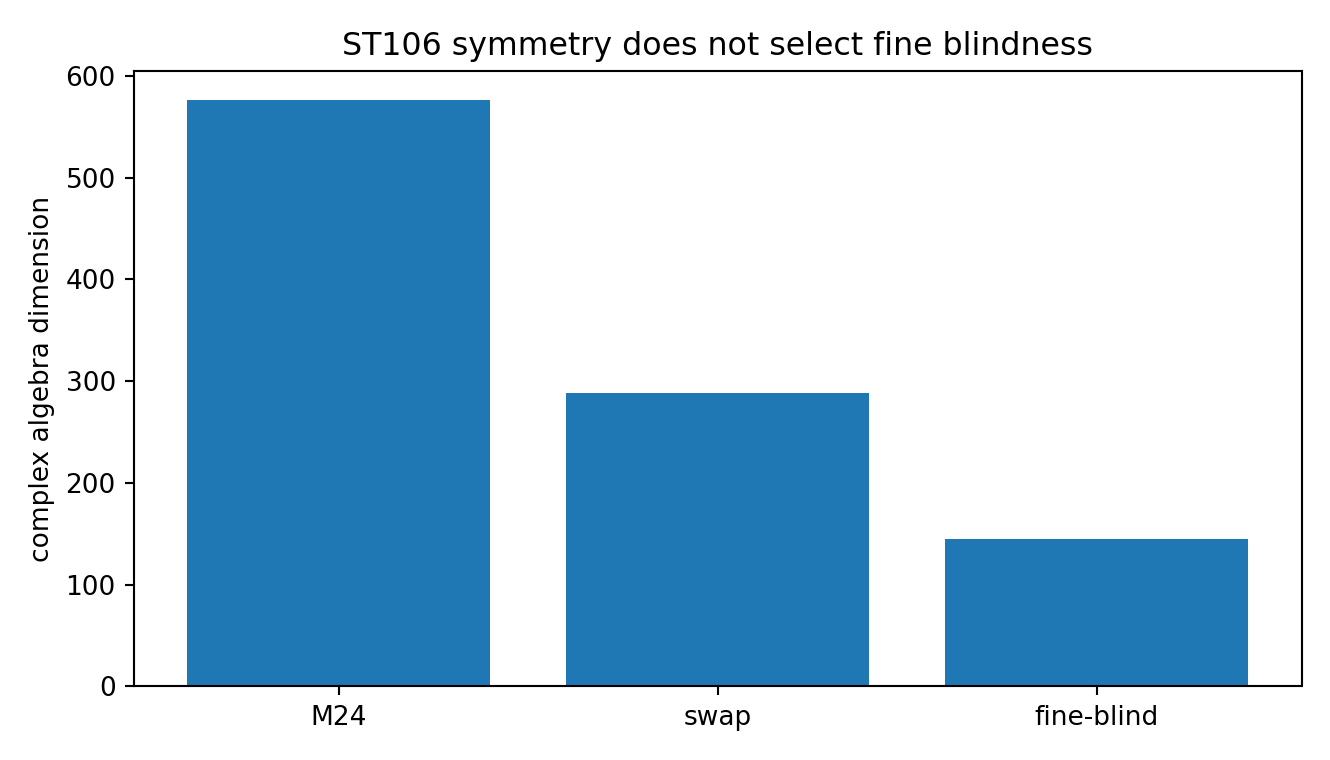
\includegraphics[width=.76\textwidth]{FIN_ST106_ST117_Figures/st106_algebra_dimensions.png}
\caption{ST106/ST114. Neither swap symmetry nor unrestricted vertex locality selects the fine-blind algebra.}
\end{figure}

\section{ST107 and ST117: exact adversarial geometry of the lift fiber}

The feasible set~\eqref{eq:fiber} lives in the $78$-dimensional real vector space of symmetric $12\times12$ matrices.

\begin{theorem}[Recession cone]
The recession cone of~\eqref{eq:fiber} is
\[
\operatorname{rec}(\mathcal F)=\{\operatorname{diag}(t_0,\ldots,t_{11}):t_i\ge0\}.
\]
Its extreme rays are the twelve rank-one rays $\mathbb R_+E_{ii}$.
\end{theorem}

\textit{Proof.} Every off-diagonal coordinate is bounded above and below, so any recession direction has $D_{ij}=0$ for $i\ne j$. A diagonal matrix is positive semidefinite exactly when all its diagonal entries are nonnegative. The extreme rays of the resulting orthant are the coordinate rays. \hfill$\square$

At $B=A$, all $12$ diagonal lower bounds and all $66$ independent off-diagonal lower bounds are active. These $78$ independent coordinate constraints force a single point, so $B=A$ is a vertex.

For each site $i$ and $t\ge0$, define
\begin{equation}
L_{i,t}=PAP^*+F(A+tE_{ii})F^*.
\label{eq:adversary}
\end{equation}
Then $L_{i,t}P=PA$, $L_{i,t}\succeq0$, and the graph-sign inequalities remain satisfied. For $t>0$ the lift is generally noncirculant and lies outside the previous one-parameter dyadic family. Yet
\[
P^*f(L_{i,t})P=f(A)
\]
for every finite spectral function $f$ defined on the blocks. Every coarse-conditioned protocol has exactly the same law, while
\[
\langle Fe_i,L_{i,t}Fe_i\rangle-\langle Fe_i,L_{i,0}Fe_i\rangle=t
\]
detects the alternative immediately if fine-site access is supplied.

\begin{figure}[H]\centering
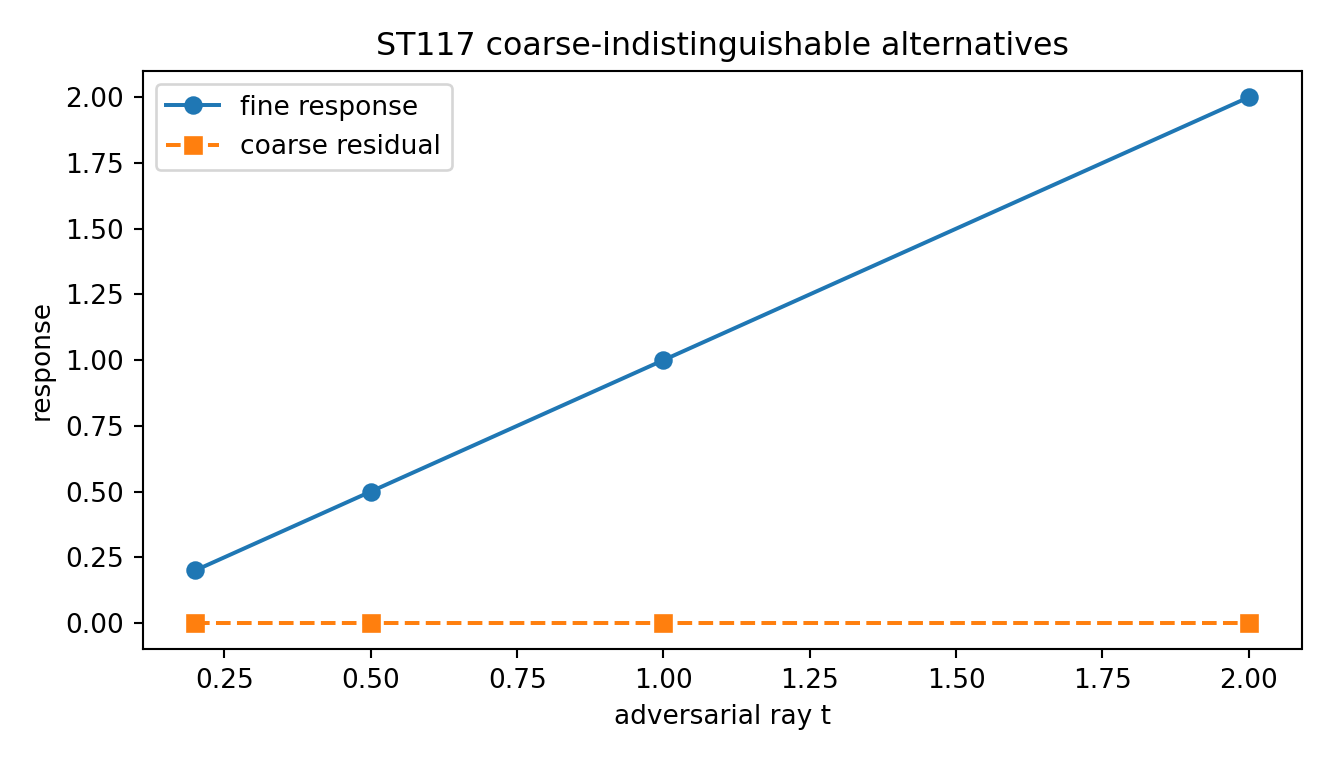
\includegraphics[width=.76\textwidth]{FIN_ST106_ST117_Figures/st117_adversarial.png}
\caption{ST117. Coarse residuals remain at floating roundoff while the declared fine observable responds linearly to the adversarial ray.}
\end{figure}

\textbf{Interpretation boundary.} This proves a hidden-model nonuniqueness theorem. It neither establishes a deeper physical layer nor selects one adversarial lift as real.

\section{ST108: interval fold theorem for the declared transcendental kernel}

The earlier ST99 calculation enclosed the frozen binary64 matrix. ST108 instead evaluates every kernel entry by outward interval arithmetic from the exact decimal/rational declaration
\[
\omega=0.18575,\qquad \phi=0.16250,\qquad \eta=\frac95.
\]
The resulting interval matrix $[A]$ is inserted directly into the reflection-reduced fold system
\[
G(q,\kappa,v;A)=0,
\]
which combines seven stationary equations, seven null-vector equations for the reduced Hessian, and $\tfrac12(v^Tv-1)=0$.

Let $x_0\in\mathbb R^{15}$ be the numerical center and $X=x_0+[-r,r]^{15}$. With a numerical inverse $C$ of the midpoint Jacobian, the parametric Krawczyk image is
\[
K(X,[A])=x_0-CG(x_0;[A])+(I-C[\partial_xG](X;[A]))(X-x_0).
\]

\begin{theorem}[Uniform parametric inclusion]
At $r=10^{-8}$ the computed Krawczyk image satisfies
\[
K(X,[A])\subset\operatorname{int}X
\]
with minimum strict margin $9.9999870606\times10^{-9}$. Therefore, for every $A$ in the interval family produced by the declared transcendental kernel formula, the fold system has one and only one root in $X$.
\end{theorem}

The theorem is parametric: the root may depend on $A$; it does not claim that all matrices share the identical root. Transcendental evaluation uses 70 decimal digits, after which outward conversion to binary64 endpoints produces propagated kernel widths of approximately one ulp ($10^{-16}$--$10^{-18}$). These wider float enclosures, not $10^{-70}$-wide stored intervals, are retained in the Krawczyk calculation.

\begin{figure}[H]\centering
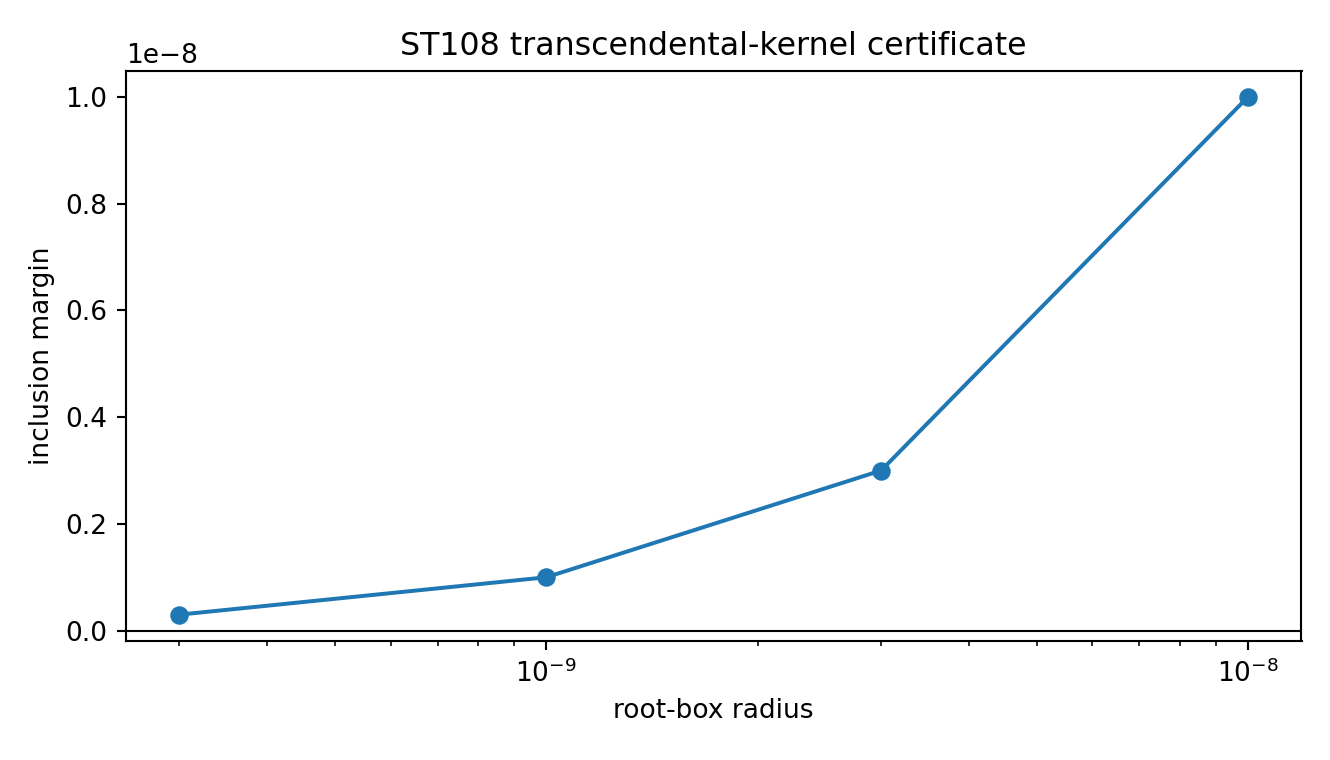
\includegraphics[width=.76\textwidth]{FIN_ST106_ST117_Figures/st108_krawczyk.png}
\caption{ST108. Strict Krawczyk inclusion remains positive when the exact-decimal transcendental kernel is interval-enclosed.}
\end{figure}

\statusboundary{} This is a reproducible source-code interval certificate. It is not independently machine-checked in a proof assistant and it does not show that a laboratory realizes the nonlinear model.

\section{ST109: maximal information recoverable after pinching}

Let $P_c=PP^*$ and $P_f=FF^*$ and consider the pinching channel
\[
\Pi(\rho)=P_c\rho P_c+P_f\rho P_f.
\]
For a code projector $Q$, the Knill--Laflamme condition for errors $P_c,P_f$ becomes
\[
QP_cQ=\alpha Q,\qquad QP_fQ=(1-\alpha)Q.
\]

\begin{theorem}[Maximal recoverable code]
The largest quantum code exactly recoverable after $\Pi$ has dimension twelve. For arbitrary $U\in U(12)$ and $0\le\alpha\le1$, it is attained by the isometry
\[
V\psi=\sqrt\alpha\,P\psi+\sqrt{1-\alpha}\,FU\psi.
\]
\end{theorem}

\textit{Proof.} Direct multiplication gives $V^*P_cV=\alpha I$ and $V^*P_fV=(1-\alpha)I$. Measuring the sector and applying the inverse branch isometry recovers the encoded state. If both branch weights are nonzero, each branch restriction is injective into a twelve-dimensional sector; hence the code dimension is at most twelve. At an endpoint the entire code lies in one such sector, with the same bound. \hfill$\square$

This is stronger than recovery of commuting reference states: every family of states on the encoded $12$-dimensional space, including noncommuting families, is recovered. It does not remove the operational premise; the encoding, sector measurement, and branch correction must all be implemented.

\section{ST110: invariant probability is not a selector}

Suppose $C_{12}$ acts transitively on twelve stable branches. Any invariant probability $\mu$ satisfies $\mu_i=\mu_{i+1}$, hence
\[
\mu_i=\frac1{12},\qquad H(\mu)=\log12=2.4849066498\ \text{nats}.
\]

\begin{theorem}[Equivariant nonselection]
The uniform law is the unique $C_{12}$-invariant branch probability. It cannot provide a canonical deterministic branch or distinguish a direction from its reflected partner.
\end{theorem}

The result clarifies spontaneous-symmetry language. Symmetry supplies a degenerate orbit of possibilities; it is not itself positive feedback. A nonuniform realized branch requires either a state/boundary perturbation, stochastic event and record, or a symmetry-breaking source. None is exported by the strict operator.

\begin{figure}[H]\centering
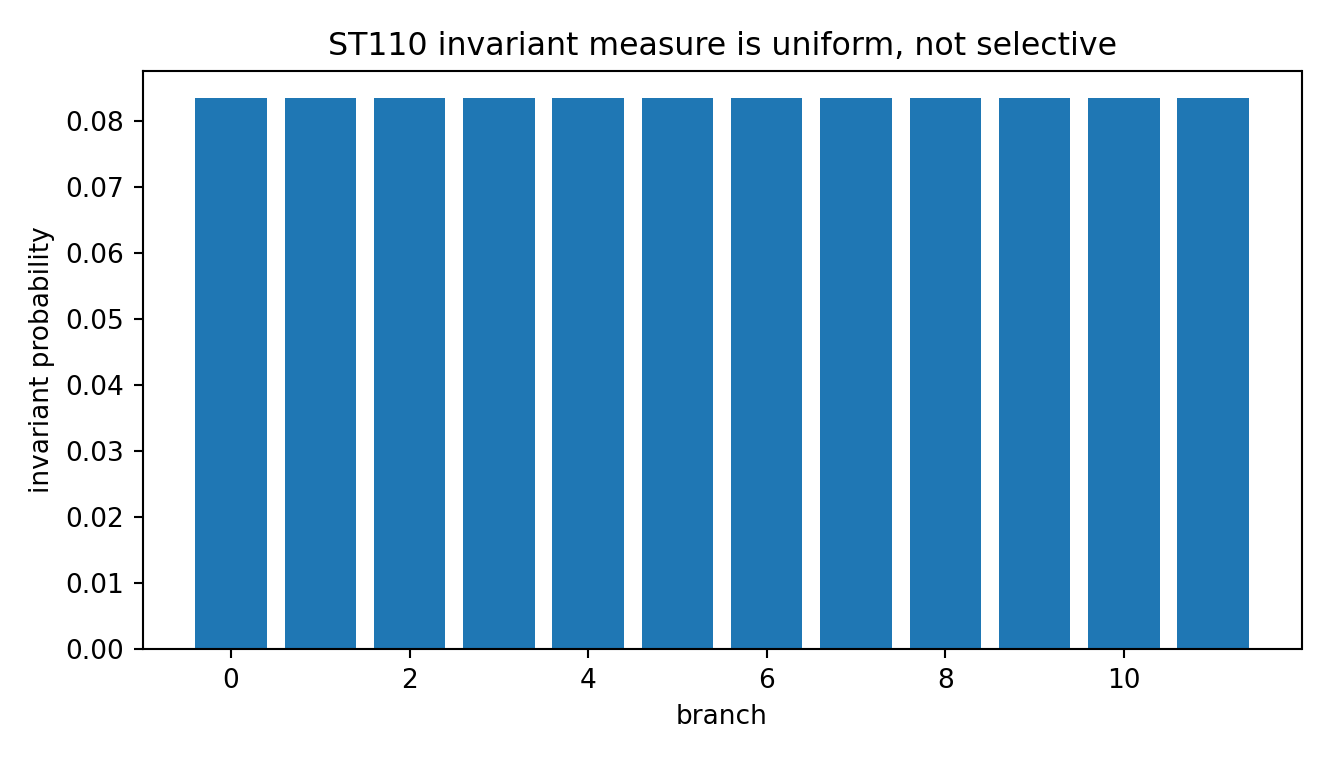
\includegraphics[width=.72\textwidth]{FIN_ST106_ST117_Figures/st110_uniform_measure.png}
\caption{ST110. Invariance fixes a uniform distribution but chooses no member of the orbit.}
\end{figure}

\openstatus{} QW-2191 remains a genuine selector obstruction.

\section{ST111: antisymmetric memory creates phase, not active gain}

Consider the collocated realization
\[
\dot x=-(S+\Omega)x+Bu,\qquad y=B^Tx,\qquad S=S^T\succ0,\quad\Omega^T=-\Omega.
\]
For $V(x)=\tfrac12x^Tx$,
\[
\dot V=-x^TSx+u^Ty,
\]
because $x^T\Omega x=0$. Thus $\Omega$ may generate circulation, complex poles, and phase delay, but does not inject energy.

The tested $2\times2$ block has $S=0.35I$ and
\[
\Omega=\begin{pmatrix}0&-1.7\\1.7&0\end{pmatrix},
\]
with poles $-0.35\pm1.7i$. Its sampled collocated transfer function has positive real part throughout $\omega\in[0,5]$.

\begin{figure}[H]\centering
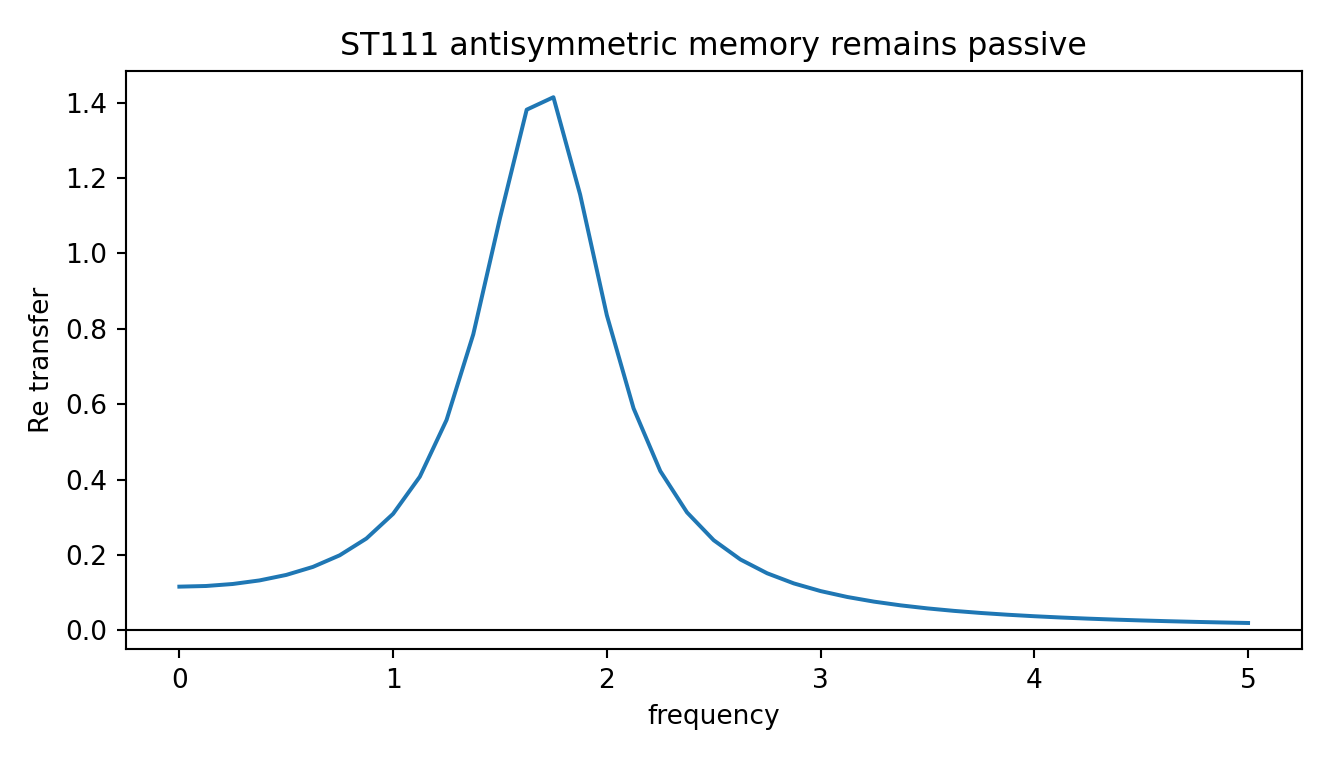
\includegraphics[width=.74\textwidth]{FIN_ST106_ST117_Figures/st111_passive_antisymmetric.png}
\caption{ST111. An antisymmetric internal block changes phase but preserves passivity.}
\end{figure}

Active amplification requires a separately sourced pump, indefinite dissipative part, nonequilibrium state, or noncollocated port accounting. Therefore an antisymmetric ``mirror coupling'' does not by itself supply the missing positive information feedback.

\section{ST112 and ST115: robust synthetic discrimination}

For the dyadic fine block $B(q)=B(0)+2qI$, the globally normalized Gibbs coarse probability is
\[
p(q;\beta)=\frac{Z_c(\beta)}{Z_c(\beta)+e^{-2\beta q}Z_f(\beta)}.
\]
With symmetric detector bit-flip probability $\delta$,
\[
p_\delta=\delta+(1-2\delta)p,
\]
and the one-event Fisher information for $q$ is exactly
\begin{equation}
\mathcal I_q=\frac{4\beta^2(1-2\delta)^2p^2(1-p)^2}{p_\delta(1-p_\delta)}.
\label{eq:fisher}
\end{equation}
For $q_0=0.2$, $q_1=0.7$, and worst declared $\delta=0.05$, a 500-point scan over $\beta\in[0.05,5]$ gives its best point near $\beta=2.18277$ and Bernoulli Chernoff information $0.0407308$. This is \strong{} because the continuous optimum was not interval-isolated.

\begin{figure}[H]\centering
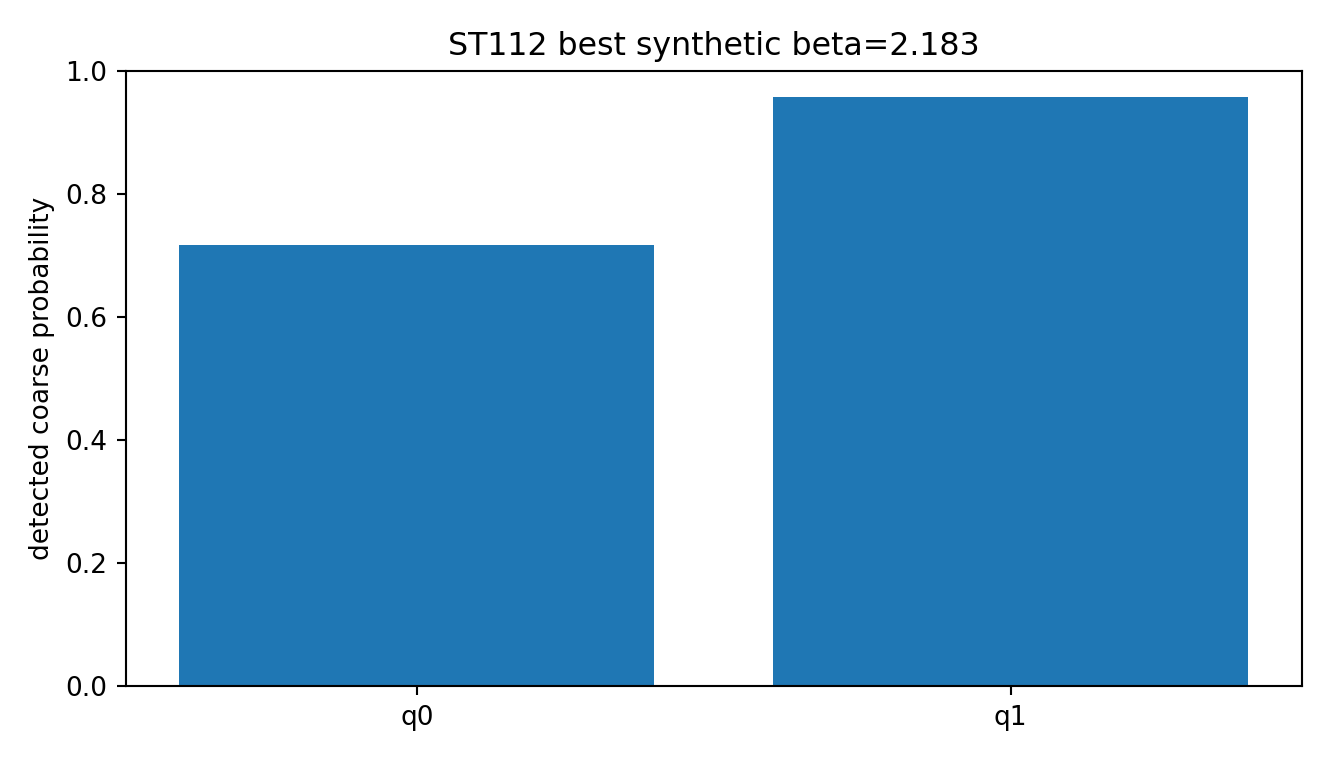
\includegraphics[width=.70\textwidth]{FIN_ST106_ST117_Figures/st112_design.png}
\caption{ST112. Conditional binary outcome separation at the best sampled inverse-temperature parameter.}
\end{figure}

ST115 addresses a different, previously open problem: independent uniform contamination of the full frozen ST87 probability tables,
\[
p_{\epsilon_P}=(1-\epsilon_P)p+\epsilon_Pu,\qquad
q_{\epsilon_Q}=(1-\epsilon_Q)q+\epsilon_Qu,
\quad (\epsilon_P,\epsilon_Q)\in[0,0.12]^2.
\]
Define the Chernoff coefficient
\[
B_s(\epsilon_P,\epsilon_Q)=\sum_jp_{\epsilon_P,j}^{s}q_{\epsilon_Q,j}^{1-s},
\qquad F=\min_{0\le s\le1}B_s,\qquad C=-\log F.
\]

\begin{theorem}[Global independent-box worst corner]
For the frozen synthetic tables, $C$ is globally minimized on $[0,0.12]^2$ at $(0.12,0.12)$. The value is
\[
C_{\rm worst}=0.0404022886255.
\]
\end{theorem}

\textit{Proof.} For each $s$, the weighted geometric mean makes $B_s$ jointly concave in its two distribution arguments. Its pointwise infimum $F$ is concave. At the upper corner, interval arithmetic isolates the unique minimizing exponent in a radius-$2\times10^{-7}$ interval around $s=0.5227767662$: the derivative is negative at the left endpoint, positive at the right endpoint, and $\partial_s^2B_s\ge0.3042373594$. The envelope derivatives satisfy
\[
\partial_{\epsilon_P}F\ge0.1268613377,
\qquad
\partial_{\epsilon_Q}F\ge0.05687236325.
\]
For every lower point $y$ in the rectangle, the supporting-hyperplane inequality for concave $F$ gives
\[
F(y)\le F(x)+\nabla F(x)\cdot(y-x)\le F(x),\qquad x=(0.12,0.12).
\]
Thus $F$ is globally maximized and $C=-\log F$ globally minimized at $x$. \hfill$\square$

\begin{figure}[H]\centering
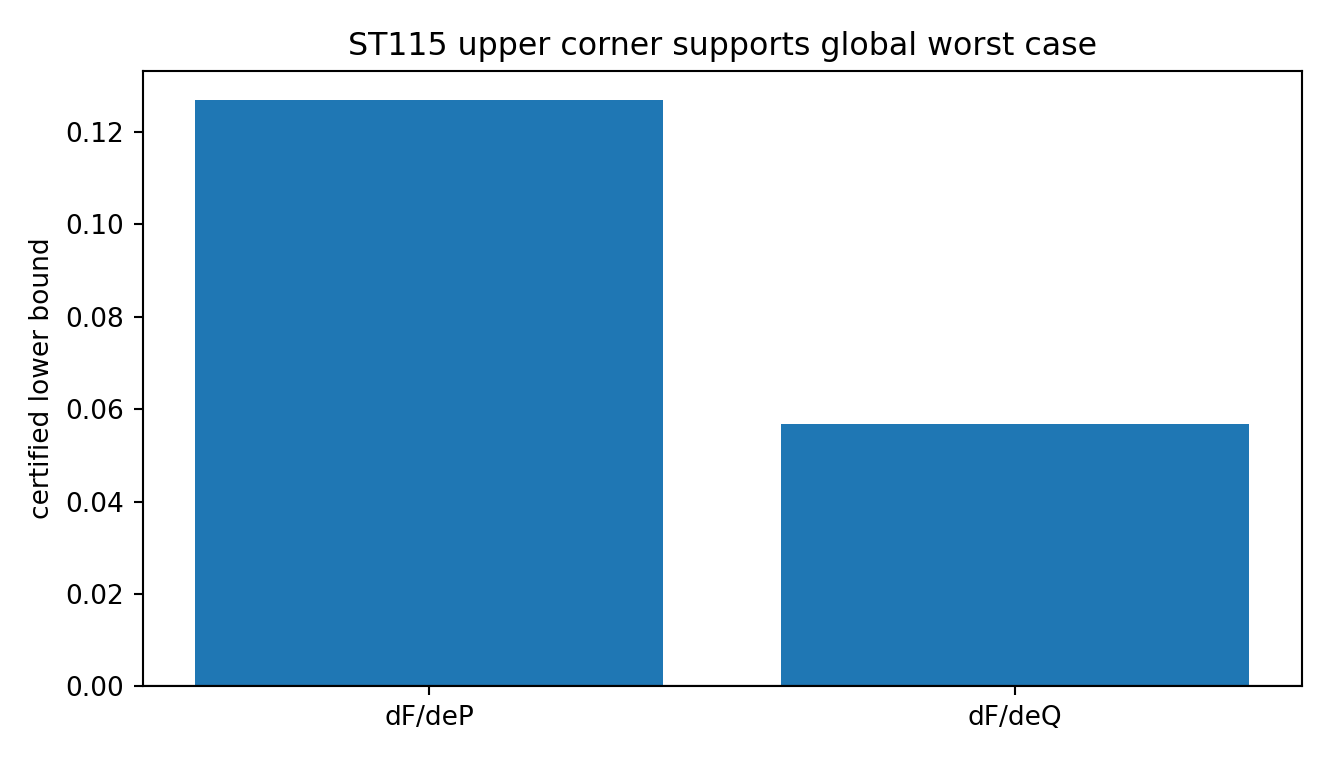
\includegraphics[width=.70\textwidth]{FIN_ST106_ST117_Figures/st115_nuisance_gradient.png}
\caption{ST115. Strictly positive certified envelope derivatives at the upper corner complete the global concavity argument.}
\end{figure}

\statusboundary{} The theorem concerns a declared uniform-contamination model and frozen synthetic probability tables. Correlated, nonuniform, drifting, or adversarial laboratory errors remain outside its scope.

\section{ST113: spin twists live on a directed refinement category}

Degree-two refinement maps are not invertible, so the correct combinatorial object is a directed category rather than a groupoid. Let $h_n\in\mathbb Z_2$ be holonomy at level $n$. Untwisted pullback gives
\[
h_{n+1}=h_n^2=+1.
\]
With a newly supplied twist $t_n\in\mathbb Z_2$,
\[
h_{n+1}=t_nh_n^2=t_n.
\]

\begin{proposition}
Through depth $L$, untwisted refinement permits only two histories and both are periodic after the first refinement. Independent twists permit all $2^{L+1}$ holonomy histories; every later holonomy equals a newly supplied twist.
\end{proposition}

This is a clean classification but a negative source result: a persistent antiperiodic/spin-like sector does not descend automatically from the scalar base. Every nontrivial refined holonomy must be provided by additional boundary data or a future twist-generating theorem.

\section{ST116: why a thermal separation was not claimed}

Covariant Gibbs-preserving (CGP) is a property of a system channel after a system Hamiltonian and $\beta$ are supplied. ``Thermal operation'' additionally refers to a dilation
\[
\Phi(\rho)=\operatorname{Tr}_B\!\left[U(\rho\otimes\gamma_B)U^*\right],
\qquad[U,H_S+H_B]=0.
\]
Whether a CGP map lies outside this class depends on the admissible bath spectra, exact or approximate dilations, ancillary dimensions, closure under limits, and possible catalysts. The current FIN artifacts declare none of these.

\begin{proposition}[Typing obstruction]
On the current artifact set, ``construct a CGP map outside thermal operations'' is under-specified: the right-hand class is not uniquely defined. Consequently no strict separation witness can be promoted without adding a bath/dilation specification.
\end{proposition}

This result is intentionally conservative. It is not evidence that CGP equals thermal operations, and it is not a thermodynamic realization of FIN. ST128 is designed to declare one finite admissible class and turn the question into exact semidefinite feasibility.

\section{Failed approaches and falsification ledger}

\begin{enumerate}
\item \textbf{Symmetry as a selector failed.} Swap symmetry retained the whole fine matrix algebra rather than erasing it.
\item \textbf{Locality as a selector failed in the opposite direction.} Vertex resolution plus connected propagation generated every matrix unit.
\item \textbf{Invariant probability did not select a realization.} It forced the uniform distribution.
\item \textbf{Antisymmetric memory did not generate active information gain.} The skew term vanished from the storage balance.
\item \textbf{Functorial spin inheritance failed.} Binary cover pullback squared holonomy to $+1$; twists remained new data.
\item \textbf{Thermal strictness was not forced.} The relevant comparison class was absent, so an apparent witness would have been definition-dependent.
\item \textbf{Dyadic uniqueness was decisively falsified.} Twelve noncirculant unbounded rays preserve all coarse records.
\item \textbf{Two earlier numerical limitations were removed.} The fold now includes the declared transcendental kernel intervals, and the independent nuisance rectangle now has a global proof.
\end{enumerate}

\section{What this batch changes in the current theory state}

The strongest positive advances are mathematical, not ontological:
\begin{itemize}
\item the nonlinear fold is no longer limited to a frozen binary64 operator;
\item the maximum quantum information recoverable after the declared pinching is classified exactly;
\item the independent contamination max--min is globally certified for its frozen synthetic model;
\item the adversarial lift directions are explicit and unbounded.
\end{itemize}

The strongest negative result is the convergence of ST106 and ST114:
\[
\boxed{\text{strict operator + swap symmetry + ordinary vertex locality}\not\Rightarrow
\text{fine-blind observable algebra}.}
\]
This does not prove that a projection principle is impossible. It proves that a missing operational equivalence relation remains necessary. Such a relation would have to explain why all fine-sector observables are identified while the coarse matrix algebra remains fully visible.

Information in this model is not merely the eigenvalue list. The adversarial lifts share every coarse spectral response but differ in fine projectors and local geometry. Any medium-independent or representation-independent FIN information object must therefore include at least the accessible algebra/channel and its intertwiners, not only the spectrum.

\section{Recommended next programs ST118--ST129}

\small
\begin{longtable}{@{}p{0.07\textwidth}p{0.57\textwidth}p{0.26\textwidth}@{}}
\toprule Priority & Program & Success criterion\\\midrule\endfirsthead
\toprule Priority & Program & Success criterion\\\midrule\endhead
1 & \textbf{ST118}: derive or obstruct fine blindness from an explicit operational equivalence relation & A universal property selecting $M_{12}\oplus\mathbb C$, or a no-go\\
2 & \textbf{ST119}: enumerate bounded faces/vertices of the lift spectrahedron under cyclic symmetry reduction & Certified face list or bounded partial classification\\
3 & \textbf{ST120}: dependency-minimal replay of ST108 & Standard-library or exact-kernel independent certificate\\
4 & \textbf{ST121}: classify all maximal recoverable codes & Normal form up to sector unitaries\\
5 & \textbf{ST122}: seek a strict-derived nonuniform invariant state without selector replay & New typed state source, or invariant no-go\\
6 & \textbf{ST123}: minimal nonpassive port/source extension & Necessary and sufficient activity condition plus cost\\
7 & \textbf{ST124}: interval-certify ST112's continuous optimum & Unique $\beta$ interval and finite-count robust design\\
8 & \textbf{ST125}: mixed-degree refinement twists & Coherent cocycle classification for nonbinary maps\\
9 & \textbf{ST126}: causal-net/code-subspace locality & Algebra-selection theorem distinct from vertex locality\\
10 & \textbf{ST127}: correlated/nonuniform contamination & Certified robust Chernoff region beyond uniform noise\\
11 & \textbf{ST128}: finite bath/dilation thermal test & Exactly typed SDP witness or equality obstruction\\
12 & \textbf{ST129}: minimax fine observable against adversarial lifts & Optimal detector over a declared bounded lift cone\\
\bottomrule
\end{longtable}
\normalsize

\section{Reproducibility}

Primary artifacts are:
\begin{itemize}
\item \texttt{fin\_st106\_st117\_research.py};
\item \texttt{test\_fin\_st106\_st117.py};
\item \texttt{FIN\_ST106\_ST117\_Results.json} and summary CSV;
\item \texttt{FIN\_ST108\_Transcendental\_Fold\_Certificate.json};
\item \texttt{FIN\_ST115\_Independent\_Nuisance\_Global\_Certificate.json};
\item \texttt{FIN\_ST117\_Adversarial\_Projection\_Alternatives.json};
\item eight generated figures and the release SHA-256 manifest.
\end{itemize}

The batch was executed under Python 3.12 with NumPy, SciPy, mpmath interval arithmetic, and Matplotlib. The test command
\[
\texttt{python3 -m unittest -v test\_fin\_st106\_st117.py}
\]
passes all 28 tests. The tests include live reconstruction of the lift vertex/ray and the Knill--Laflamme identities, not only reads from frozen JSON.

The ST108 proof uses 70-decimal-digit interval evaluation for the transcendental kernel and outward \texttt{nextafter} enclosure around binary64 linear algebra. The ST115 certificate records the interval signs, curvature, envelope derivatives, model, seed-derived probability tables, and worst-corner value. These are auditable computational theorems in source-code scope, not formal proof-assistant exports.

\section{Final verdict}

\resultbox{\textbf{Verdict surviving this falsification round.} The FIN projection architecture is a mathematically coherent family of coarse-grainings and recoverable codes over a much larger hidden spectrahedral lift space. It is not selected by the currently declared strict operator: swap symmetry leaves too much fine structure, vertex locality exposes all of it, invariant probability chooses no branch, and refinement generates no spin twist. The theory has gained two proof-grade closures---the transcendental-kernel fold and the independent-nuisance worst corner---but the bridge from this finite operator mathematics to a unique physical observable world remains an explicit missing operational principle.}

The smallest credible next target is not another analogy. It is a theorem or obstruction showing whether a declared operational equivalence relation can uniquely select the fine-blind algebra while remaining compatible with composition, recovery, and falsification. Until then, the projected-universe interpretation is an organized research hypothesis, not a consequence of strict FIN and not experimentally established physics.

\begin{thebibliography}{9}
\bibitem{Krawczyk} R. Krawczyk, ``Newton-Algorithmen zur Bestimmung von Nullstellen mit Fehlerschranken,'' \emph{Computing} 4 (1969), 187--201.
\bibitem{KnillLaflamme} E. Knill and R. Laflamme, ``Theory of quantum error-correcting codes,'' \emph{Physical Review A} 55 (1997), 900--911.
\bibitem{Petz} D. Petz, ``Sufficiency of channels over von Neumann algebras,'' \emph{Quarterly Journal of Mathematics} 39 (1988), 97--108.
\bibitem{Chernoff} H. Chernoff, ``A measure of asymptotic efficiency for tests of a hypothesis based on the sum of observations,'' \emph{Annals of Mathematical Statistics} 23 (1952), 493--507.
\bibitem{BratteliRobinson} O. Bratteli and D. W. Robinson, \emph{Operator Algebras and Quantum Statistical Mechanics I}, Springer, second edition, 1987.
\end{thebibliography}

\end{document}
